\chapter{Cinetica}
La termodinamica dice tutto relativamente alla spontaneità di una reazione o di un processo chimico, tuttavia un processo termodinamicamente favorevole può avvenire con una lentezza tale per cui praticamente non è osservabile. In questi casi si dice che il
processo è cineticamente sfavorevole.
\section{Velocità di reazione}
Considerando una generica reazione
\begin{equation}
    \alpha A+\beta B\to\gamma C,
\end{equation}
e considerando le concentrazioni [A], [B] e [D], la velocità con cui varia una data specie, ovvero la variazione della concentrazione nel tempo, misura la velocità istantanea della reazione
\begin{equation}
    -\frac{1}{\alpha}\frac{d[A]}{dt}=-\frac{1}{\beta}\frac{d[B]}{dt}=\frac{1}{\gamma}\frac{d[C]}{dt},
\end{equation}
In cui il segno ``–'' indica il fatto che i reagenti si consumano man mano che la reazione procede.

Sperimentalmente si constata che la velocità misurata in un certo istante, risulta proporzionale alla concentrazione dei reagenti (a volte anche a quella dei prodotti) elevate a dei coefficienti, che non sono i coefficienti stechiometrici. Ad esempio, in questo caso potrebbe essere
\begin{equation}
    v_A=-\frac{d[A]}{dt}=-k[A]^a[B]^b,
\end{equation}
ed eventualmente anche
\begin{equation}
    v_A=-\frac{d[A]}{dt}=-k[A]^a[B]^b[C]^c.
\end{equation}
Questa equazione, determinata per via empirica, prende il nome di equazione cinetica. La costante $k$ viene indicata come costante cinetica ed è indipendente dalle concentrazioni, mentre dipende dalla temperatura. Oltre a permettere di prevedere la velocità di reazione, questa equazione  permette di classificare le reazioni in base al rispettivo ordine.
\begin{defn}[ordine di un componente di una reazione]
    L'ordine relativo ad un certo componente, è l'esponente al quale la concentrazione di quel componente è elevata nell'equazione cinetica. L'ordine complessivo è dato dalla somma degli ordini dei singoli componenti. 
\end{defn}

\section{Costante cinetica}
Aumentando la temperatura si osserva che la specifica equazione cinetica resta per lo più invariata ma la costante cinetica $k$ aumenta in modo significativo. L'osservazione empirica rende lecita la seguente equazione
\begin{equation}
    k=Ae^{E_a/RT}.
\end{equation}
Questa equazione prende il nome di equazione di Arrhenius, in cui $E_a$ è l'energia di attivazione. Da questa si può vedere che la relazione tra $\ln{k}$ e $1/T$ è lineare. Sempre in questa equazione l'energia cinetica rappresenta l'energia necessaria per far avvenire la reazione, mentre il termine $RT$ rappresenta l'energia disponibile nell'ambiente. In base alla distribuzione di Boltzmann, a temperatura $T$, la proporzione degli urti efficaci vale proprio $e^{E_a/RT}$. Più alta è la temperatura, maggiore è il numero di urti.

Se l'ordine di reazione coincide con la stechiometria di reazione (fatto non sempre verificato) è possibile scrivere
\begin{equation}
    \frac{k_d}{k_i}=K_{eq},
\end{equation}
dove $k_d$ indica la costante cinetica della reazione diretta e $k_i$ indica la costante cinetica della reazione inversa. Ora 
\begin{equation}
    K_{eq}=e^{-\Delta G^\circ/RT}=\frac{A_d}{A_i}\exp{\bigg(-\frac{E_{(a,d)}-E_{(a,i)}}{RT}\bigg)}.
\end{equation}
Per definizione, $\Delta G^\circ=\Delta H^\circ-T\Delta S^\circ$, quindi passando ai logaritmi si ottiene
\begin{equation}\label{eq:entalp.+entrop.}
    -\frac{\Delta H^\circ}{RT}+\frac{\Delta S^\circ}{R}=-\frac{E_{(a,d)}-E_{(a,i)}}{RT}+\ln{\frac{A_d}{A_i}}.
\end{equation}
Dato che in entrambi i membri dell'equazione è contenuto un termine fortemente dipendente dalla temperatura e un termine in cui la dipendenza dalla temperatura è trascurabile. Il primo e il terzo termine devono essere uguali come il secondo e l'ultimo
\begin{equation}\label{eq:sistema entalp. entrop.}
    \begin{cases}
        \dfrac{\Delta H^\circ}{RT}=\dfrac{E_{(a,d)}-E_{(a,i)}}{RT} \\[2ex]
        \dfrac{\Delta S^\circ}{R}=\ln{\dfrac{A_d}{A_i}}.
    \end{cases}
\end{equation}

\subsection{Significato della parte energetica}
La prima equazione del sistema \eqref{eq:sistema entalp. entrop.}  non coinvolge necessariamente il termine $RT$ e può essere scritta come
\begin{equation}
    \Delta H^\circ=E_{(a,d)}-E_{(a,i)}.
\end{equation}
Nella reazione diretta, i reagenti sono ad un'entalpia intrinseca $H_1$ e devono superare una barriera entalpica che corrisponde all'entalpia di attivazione $\Delta H_d^\#=E_{(a,d)}$ per arrivare ai prodotti. In quella inversa i prodotti sono ad un'entalpia intrinseca $H_2$ devono superare una barriera entalpica $\Delta H_i^\#=E_{(a,i)}$. Osservando il diagramma si deduce che la barriera è la stessa, quindi
\begin{equation}\label{eq:H2-H1}
    H_2-H_1=\Delta H_d^\#-\Delta H_i^\#=E_{(a,d)}-E_{(a,i)}=\Delta H^\circ.
\end{equation}
\begin{figure}[h]
    \centering
    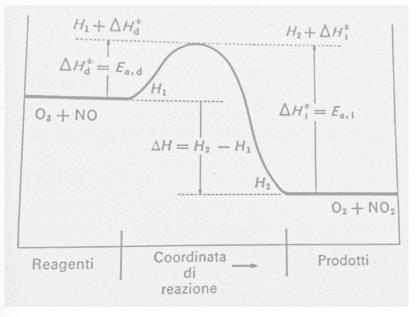
\includegraphics[width=0.5\linewidth]{Immagini/Barriera entalpica.png}
    \caption{barriera entalpica.}
    \label{fig:e}
\end{figure}

\subsection{Significato della parte entropica}
Il fattore pre esponenziale  $A$ dell'equazione di Arrhenius è un termine di probabilità.  Esso misura la probabilità che ha una collisione di avere una particolare energia e geometria efficacie. La seconda equazione del sistema \eqref{eq:sistema entalp. entrop.} può essere scritta come
\begin{equation}\label{eq:Sstd}
    \Delta S^\circ=R\ln{\frac{A_d}{A_i}}=R\ln{A_d}-R\ln{A_i}.
\end{equation}
Questo risultato è riconducibile all'espressione di Boltzmann per l'entropia $S=k\ln{\omega}$ per cui la seconda equazione del sistema \eqref{eq:sistema entalp. entrop.} può essere interpretata in termini di un'entropia di attivazione.

E' evidente quindi che il processo di attivazione è caratterizzato da una barriera che ostacola e controlla
il procedere della reazione e in questo processo è anche coinvolto un fattore legato all'entropia. Con
questo in mente possiamo tornare all'equazione \eqref{eq:entalp.+entrop.} dell'energia libera ricavata riscrivendola come
\begin{equation}
    \Delta G^\circ=(E_{(a,d)}-E_{(a,i)})-RT\ln{\frac{A_d}{A_i}},
\end{equation}
da cui, sostituendo le equazioni \eqref{eq:H2-H1} e \eqref{eq:Sstd} si ottiene
\begin{equation}
    \Delta G^\circ=(\Delta H_d^\#-T\Delta S_d^\#)-(\Delta H_i^\#-T\Delta S_i^\#).
\end{equation}
\begin{figure}[ht]
    \centering
    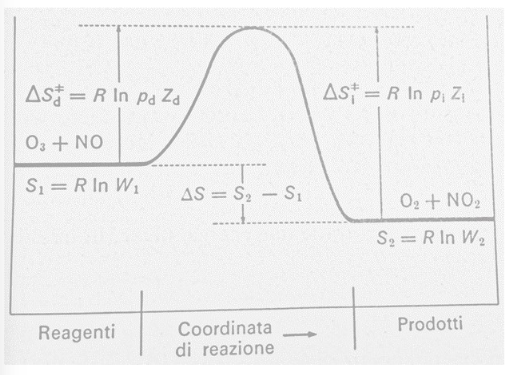
\includegraphics[width=0.5\linewidth]{Immagini/Barrieira entropica.png}
    \caption{barriera entropica.}
    \label{fig:ent}
\end{figure}

Per riassumere, la velocità con cui avviene una reazione è quindi determinata dalla necessità di superare una barriera, nello scenario dell'energia libera. Questa barriera è in parte dovuta ad un termine entalpico ed in parte ad un termine entropico. L'equilibrio è determinato da un bilancio tra la variazione di entalpia del sistema e la variazione di disordine durante la reazione. Il valore minimo di $\Delta H-T\Delta S$ per il sistema, corrisponde al massimo valore di entropia per l'universo.

Un minimo di energia libera per un sistema comporta equilibrio perché corrisponde al massimo disordine nell'universo. Nel processo di superamento della barriera, quando l'energia libera aumenta, il disordine dell'universo deve diminuire! L'universo è in continua trasformazione, è un sistema dinamico, e la condizione di disordine massimo è mantenuta statisticamente, mentre localmente e in un qualche istante di tempo, ci possono (devono) essere fluttuazioni rispetto allo stato più probabile. Per superare la barriera di energia libera, è necessaria una diminuzione momentanea nel disordine dell'universo, contraria all'andamento generale delle cose.

Si può essere certi che, aspettando un tempo sufficientemente lungo, prima o poi il disordine cospirerà inconsapevolmente per fornire la configurazione e l'energia necessaria a far avvenire la reazione.
\begin{figure}[h]
    \centering
    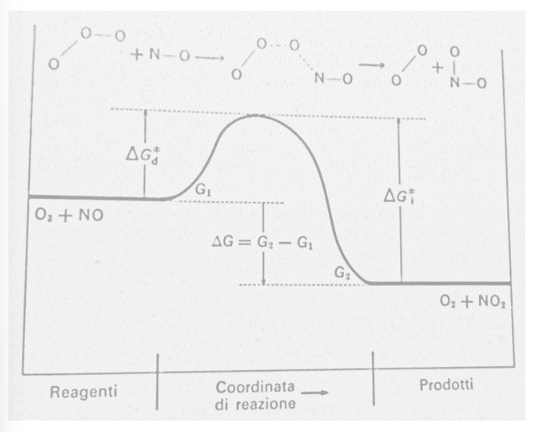
\includegraphics[width=0.5\linewidth]{Immagini/Barriera di energia libera.png}
    \caption{barriera di energia libera.}
    \label{fig:g}
\end{figure}

\section{Ordini di reazione}
\paragraph{Reazione del prim'ordine.} Una reazione del prim'ordine è una reazione in cui l'esponente a cui è elevata la concentrazione è pari a uno. L'equazione cinetica per la scomparsa di un generico reagente A è
\begin{equation}
    v_A=\frac{d[A]}{dt}=-k[A].
\end{equation}
\'E possibile integrare questa equazione, e sapendo anche che a $t=0$ la concentrazione di $A$ è $[A]_0$ si ha
\begin{equation}
    \int_{[A]_0}^{[A]}\frac{d[A]}{[A]}=-\int_{t_0}^tkdt,
\end{equation}
da cui si ottiene
\begin{equation}
    \ln{\frac{[A]}{[A]_0}}=-kt.
\end{equation}
\begin{defn}[tempo di dimezzamento]
    Il tempo di dimezzamento $t_{1/2}$ è il tempo necessario affinché la concentrazione iniziale di un generico reagente A si riduca del 50\%, ovvero $[A]/[A]_0=50\%$, dato da
    \begin{equation}
        t_{1/2}=\frac{\ln{2}}{k}.
    \end{equation}
\end{defn}
\begin{obs}
    Il tempo di dimezzamento è indipendente dalla concentrazione iniziale, per cui conoscendone il valore e misurando la concentrazione del reagente al generico tempo $t$ è possibile ricavare il tempo trascorso dall'inizio della reazione.
\end{obs}

\paragraph{Reazione del secondo ordine.} Una reazione del secondo ordine è una reazione in cui l'esponente a cui è elevata la concentrazione è pari a due. L'equazione cinetica per la scomparsa di un generico reagente A è
\begin{equation}
    v_A=\frac{d[A]}{dt}=-k[A]^2.
\end{equation}
La quale può essere integrata ottenendo
\begin{equation}
    \int_{[A]_0}^{[A]}\frac{d[A]}{[A]^2}=-\int_{t_0}^tkdt,
\end{equation}
da cui
\begin{equation}
    \frac{1}{[A]}-\frac{1}{[A]_0}=kt.
\end{equation}
Da questa equazione si vede come riportando in diagramma $1/[A]$ in funzione del tempo si ottiene una dipendenza lineare in cui la pendenza della retta fornisce il valore della costante cinetica.